%!TEX program = xelatex
 % 使用 ctexart 文类,UTF-8 编码
 % 作者:王泽宇
\documentclass[UTF8]{ctexart}
\usepackage{tikz,mathpazo}
\usetikzlibrary{shapes.geometric, arrows}
\usetikzlibrary{calc}
\usepackage{geometry}
\geometry{left=1cm, right=1cm, top=1cm, bottom=1.1cm}
\pagestyle{plain}
\usepackage{graphicx}





\title{数据结构:祖玛}
\author{17电科鲁国锐}
\begin{document}
	\maketitle
	
	\section{问题描述}
	
	
	\section{解决方案}
	
	\section{算法设计}
	

\newpage
\thispagestyle{empty}
 % 流程图定义基本形状
\tikzstyle{startstop} = [rectangle, rounded corners, minimum width=3cm, text width=2cm, minimum height=1cm,text centered, draw=black, fill=red!30]
\tikzstyle{io} = [trapezium, trapezium left angle=70, trapezium right angle=110, minimum width=3cm, text width=2cm, minimum height=1cm, text centered, draw=black, fill=blue!30]
\tikzstyle{process} = [rectangle, minimum width=3cm, text width=2cm, minimum height=1cm, text centered, draw=black, fill=orange!90]
\tikzstyle{decision} = [diamond, minimum width=3cm, text width=2cm, minimum height=1cm, text centered, draw=black, fill=green!30]
\tikzstyle{arrow} = [thick,->,>=stealth]

\begin{tikzpicture}[node distance=1.5cm, centered]
 %定义流程图具体形状
\node (start) [startstop] {开始};
\node (in1) [io, below of=start] {输入字符串balls};
\node (in2) [io, below of=in1] {输入操作数n};
\node (dec1) [decision, below of=in2, yshift=-1cm] {n>0?};
\node (iostart) [io, below of=dec1, yshift=-1cm] {输入插入位置start};
\node (ioball) [io, below of=iostart] {输入插入球种类ball};
\node (insert) [process, below of=ioball] {balls
	.insert(start,ball)};
\node (find) [process, below of=insert] {end=
	find(start,balls)};
\node (whileablat)[decision, below of=find, yshift=-1.5cm]{ablat(sta
	rt,end,balls)?};
\node (find2)[process, below of=whileablat, yshift=-1.5cm] {end=
	find(start,balls)};
\node (out)[io, below of=find2, yshift=-0.45cm]{输出balls,若为空则输出'-'};
\node (nd)[process, below of=out, yshift=-0.25cm]{n--};
\node (end) [startstop, below of=nd] {结束};


\node (findstart) [startstop, right of=start, xshift=5.5cm] {开始};
\node (findinput) [io, below of=findstart, yshift=-0.5cm] {传入start的引用, balls};
\node (findleft) [decision, below of=findinput, yshift=-2.5cm]{left>=0\\
\&\&
balls[left]=
=balls[start]?};
\node (leftd) [process, below of=findleft, yshift=-2cm]{left--};
\node (findright) [decision, below of=leftd, yshift=-2cm]{right<balls.size\\
	\&\&
	balls[right]=
	=balls[start]?};
\node (righta) [process, below of=findright, yshift=-2cm]{right++};
\node (prostart)[process, below of=righta]{start=++left};
\node (findout)[io, below of=prostart]{输出right};




\node (ablatstart) [startstop, left of=start, xshift=-5.5cm] {开始};

%\node (pro2b) [process, right of=dec1, xshift=3cm] {process};

%\node (stop) [startstop, below of=ioball, yshift=-3.5] {startstop};

 %连接具体形状
 \draw ($(start.north)$) node[anchor=south]{主函数};
\draw [arrow](start) -- (in1);
\draw [arrow](in1) -- (in2);
\draw [arrow](in2) -- (dec1);
\draw [arrow](dec1) -- (iostart);
%\draw [arrow](dec1) -- (pro2b);
\draw [arrow](dec1) -- node[anchor=east] {yes} (iostart);
%\draw [arrow](dec1) -- node[anchor=south] {no} (pro2b);
%\draw [arrow](pro2b) |- (in2);
\draw [arrow](iostart) -- (ioball);
\draw [arrow](ioball) -- (insert);
\draw [arrow](insert) -- (find);
\draw [arrow](find) -- (whileablat);
\draw [arrow](whileablat) -- ($(whileablat.south)+(0,-0.2)$) node[anchor=east]{yes} -- (find2);
\draw [arrow](find2) -- ($(find2.west)+(-0.5, 0)$) node[anchor=south]{} |- ($(whileablat.west)$);
\draw [arrow](out) -- (nd);
\draw [arrow](whileablat) -- ($(whileablat.east)+(0.5,0)$) node[anchor=south]{no} |- ($(out.east)$);
\draw [arrow](nd) -- ($(nd.west)+(-1,0)$) node[anchor=south]{} |- ($(dec1.west)$);
\draw [arrow](dec1) -- ($(dec1.east)+(1,0)$) node[anchor=south]{no} |- ($(end.east)$);




%\draw [arrow](find) -- ($(find.east) + (2,0)$) node[anchor=north]{} |- (findstart);
\draw ($(findstart.north)$) node[anchor=south]{find函数};
\draw [arrow](findstart) -- (findinput);
\draw [arrow](findinput) -- (findleft);
\draw [arrow](findleft) -- ($(findleft.south) + (0, -0.3)$) node[anchor=east]{yes} -- (leftd);
\draw [arrow](leftd) -- ($(leftd.east)+(1.5,0)$) |- ($(findleft.east)$);
\draw [arrow](findleft) -- ($(findleft.west) + (-0.5, 0)$) node[anchor=south]{no} |- ($(findright.west)$);
\draw [arrow](findright) -- ($(findright.south)+(0,-0.3)$) node[anchor=east]{yes} -- (righta);
\draw [arrow](findright) -- ($(findright.east) + (0.5, 0)$) node[anchor=south]{no} |- ($(prostart.east)$);
\draw [arrow](righta) -- ($(righta.west)+(-1.30, 0)$) node[anchor=north]{} |- ($(findright.west)$);
\draw [arrow](prostart) -- (findout);




\draw ($(ablatstart.north)$) node[anchor=south]{ablat函数};

\end{tikzpicture}

\newpage


\begin{figure}[htbp] 
	\centering 
	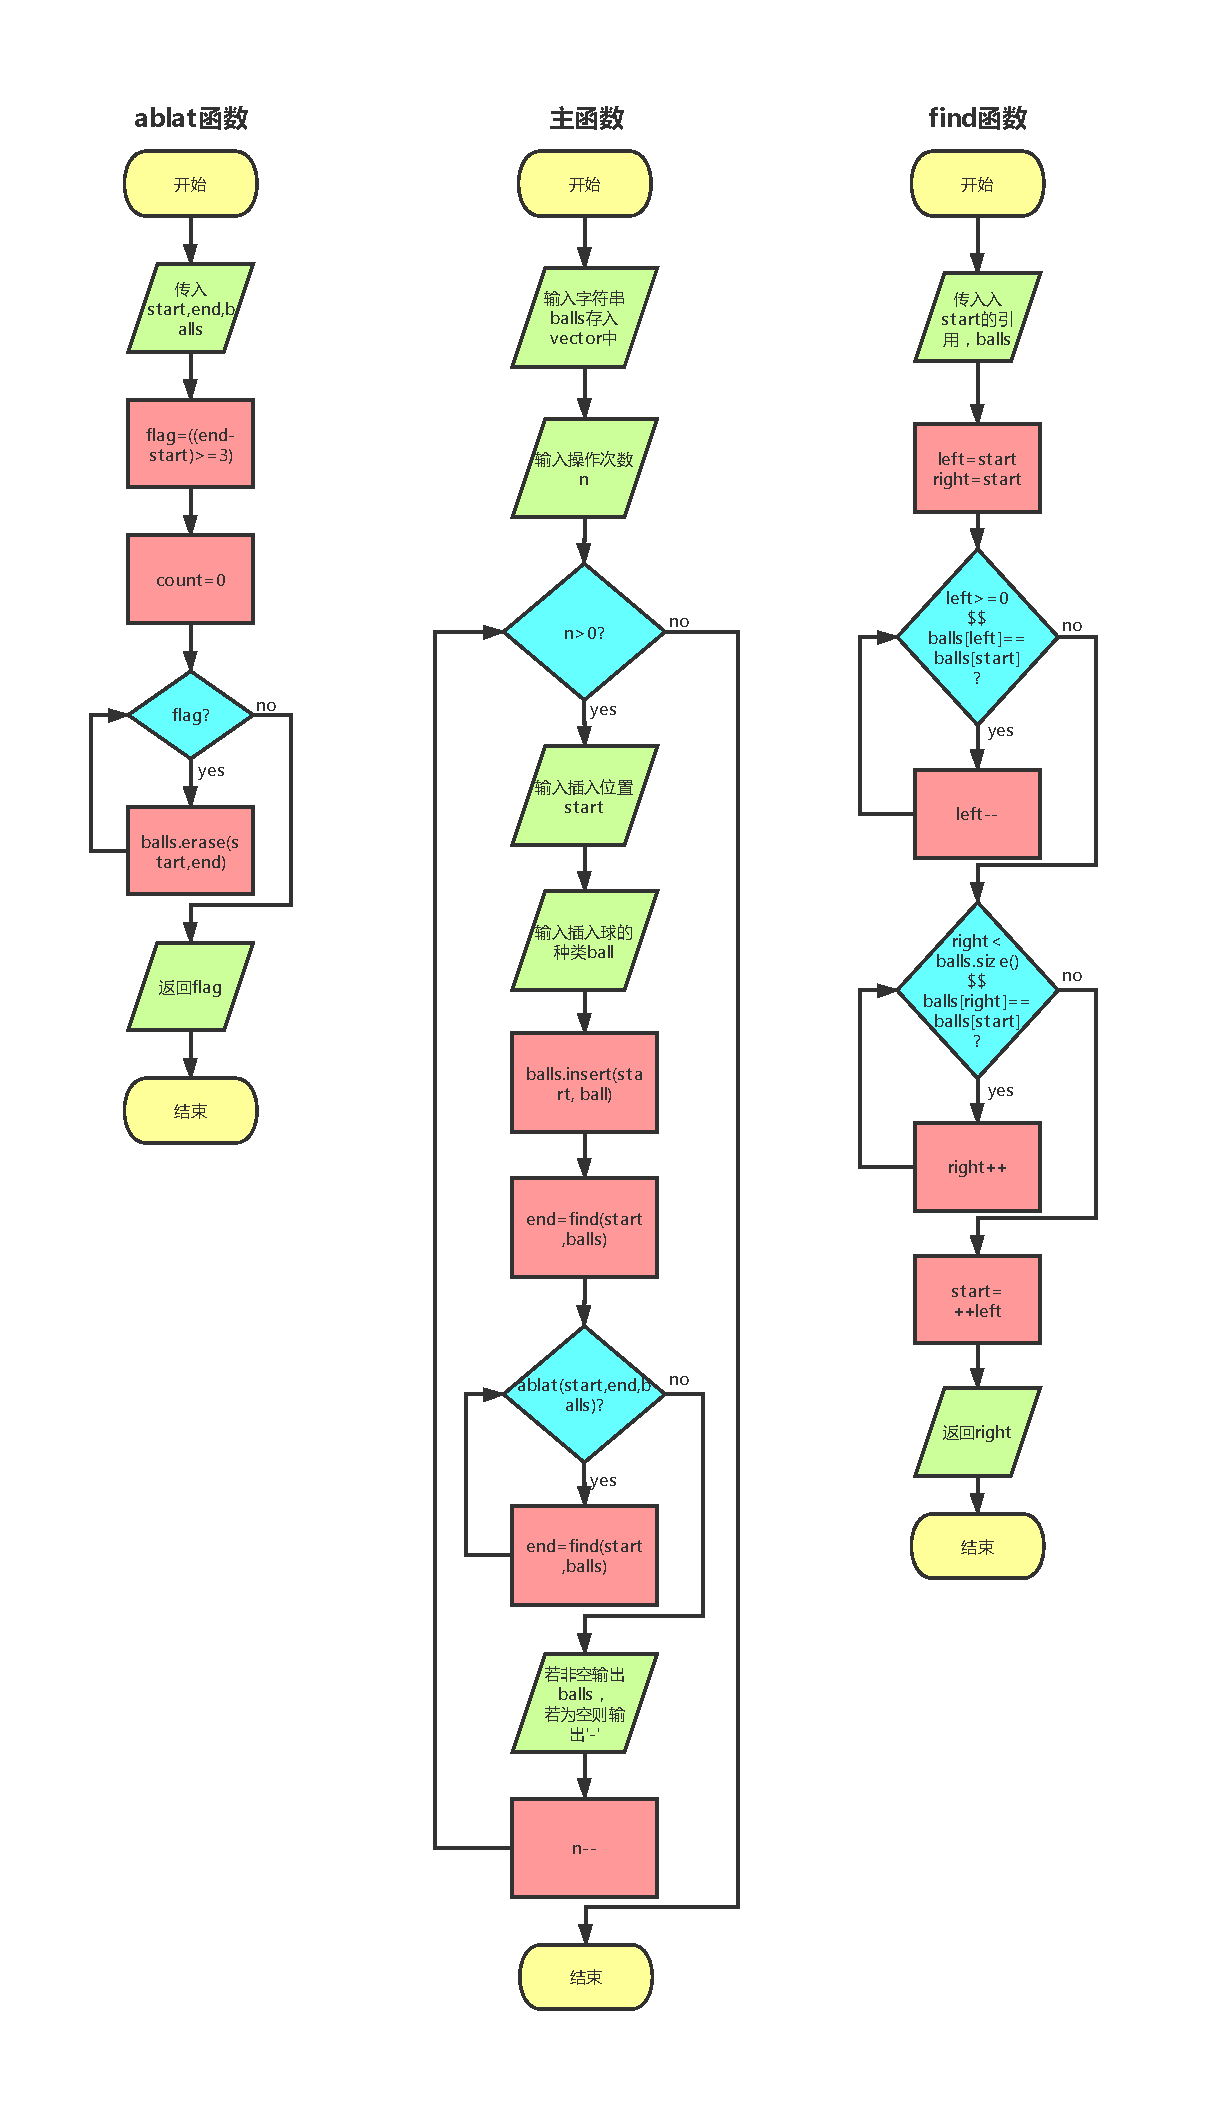
\includegraphics[scale=0.7]{zuma.pdf} 
	\caption{Design} 
\end{figure}


	\section{编程实现}
	
	\section{结果分析}
	
	\section{总结体会}


\end{document}